\documentclass[border=8pt]{standalone}
\usepackage[T1]{fontenc}\usepackage[utf8]{inputenc}\usepackage{lmodern}
\usepackage{tikz}\usetikzlibrary{arrows.meta,positioning}
\begin{document}
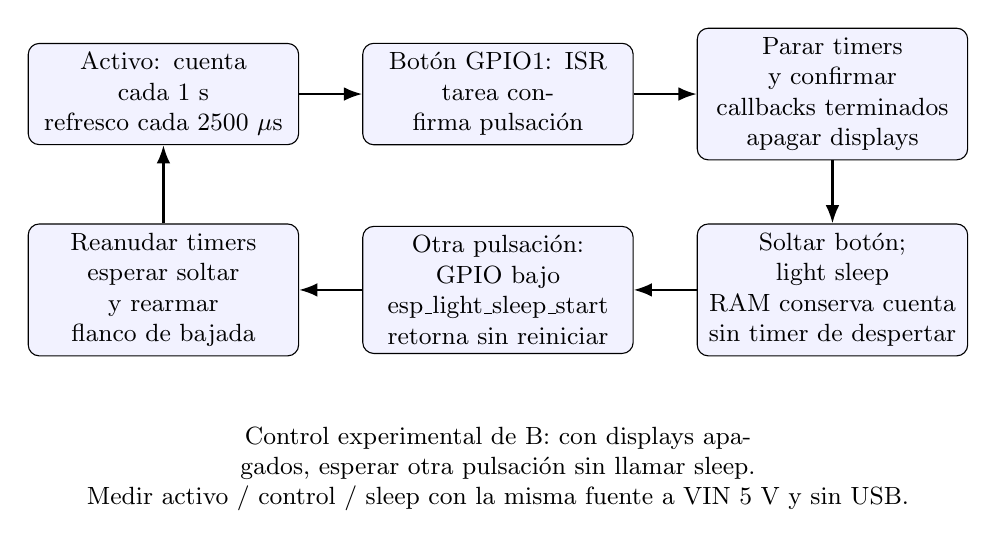
\begin{tikzpicture}[>=Latex,font=\small,node distance=0.8cm,
 b/.style={draw,rounded corners,fill=blue!5,text width=3.2cm,align=center,minimum height=1.2cm}]
\node[b] (run) {Activo: cuenta cada 1 s\\refresco cada 2500 $\mu$s};
\node[b,right=of run] (btn) {Botón GPIO1: ISR\\tarea confirma pulsación};
\node[b,right=of btn] (stop) {Parar timers y confirmar\\callbacks terminados\\apagar displays};
\node[b,below=of stop] (sleep) {Soltar botón; light sleep\\RAM conserva cuenta\\sin timer de despertar};
\node[b,left=of sleep] (wake) {Otra pulsación: GPIO bajo\\esp\_light\_sleep\_start\\retorna sin reiniciar};
\node[b,left=of wake] (resume) {Reanudar timers\\esperar soltar y rearmar\\flanco de bajada};
\draw[->,thick] (run)--(btn);\draw[->,thick] (btn)--(stop);\draw[->,thick] (stop)--(sleep);
\draw[->,thick] (sleep)--(wake);\draw[->,thick] (wake)--(resume);\draw[->,thick] (resume)--(run);
\node[below=0.8cm of wake,text width=11cm,align=center] {Control experimental de B: con displays apagados, esperar otra pulsación sin llamar sleep.\\Medir activo / control / sleep con la misma fuente a VIN 5 V y sin USB.};
\end{tikzpicture}
\end{document}
